\documentclass{article}
\usepackage{graphicx}
\usepackage{subcaption}

\title{Challenges in chaotic time series forecasting}
\author{Maximilian Hornung}

\begin{document}
\maketitle

\begin{abstract}
  Predicting the future development of time series is of interest in different
  areas of computational biology. The time series in biological models exhibit
  challenging characteristics such as chaotic or stochastic behavior. In this
  report, time series prediction is done on different kind of biological time
  series using deep neural networks. In our evaluation, we identify challenges
  and limitations of this approach, and compare different architectures of
  deep neural networks with regard to their performance.
\end{abstract}

\section{Introduction}

In various kind of diseases, it is important to choose the correct treatment at
the current time point. Since the human body is too complex to be described
directly using mathematics, special features are modeled with mathematical
systems such as the Mackey-Glass equations for respiratory and hematopoietic
diseases \cite{mackey1977}. These models make use of available data about
previous information in order to reduce the uncertainty under which a decision
is done. This is especially important when the consequences of a decision are
severe, for example the decision of breast cancer treatment after radiation.
This particular problem can be addressed by using a stochastic differential
equation, as done by Oroji \textit{et al} \cite{oroji2016}.

In different kinds of biological models, chaotic behavior is observed. Even the
Mackey-Glass equations obtain chaotic behavior for certain choices of their
parameters, as shown by Fischer \cite{farmer1982}. That means that even small
perturbations of the time series prediction increase exponentially, which means
that the time series prediction should be as robust as possible against noise.

This gets imporant in particular because another characterstic of dealing with
biological data is the presence of noise. In
this report, we show that different kinds of noise assumptions can impact the
results of time series prediction. We evaluate all our investigated problems
with regard to the popular $i.i.d.$ random noise as well as memorizing random
noise. Since mathematical models of biological systems can not describe their
characteristics perfect and error-free, it is assumed that the latter type of
noise is more realistic. But unfortunately this kind of noise increases the
difficulty of time series prediction, even for simple mathematical functions,
as seen in section~\ref{sec:sine}.

The remaining report is structured as follows. First, we perform proper time
series prediction on the $sine$ function and show how different noise models
impact the prediction ability of our network models. We conduct an evaluation
how these results can be extended to the prediction of
ordinary differential equations (\textbf{ODE}s) at the example of the
differential equations of the harmonic oscillator. After that, we show how the
stochasticity of noise impactss the possibility to predict deterministic
chaotic time series at the example of the \emph{Mackey Glass} time series. Last
but not least, we report how the poor results of numerical approximations on
stocastic differential equations (\textbf{SDE}s) can be explained based on our
previous results.

\section{Methods}

In our analysis, we use four different architectures and neural networks and
optimize their hyperparameters for the respective use case. Since Hornik
\textit{et al.} have shown that feedforward neural networks are universal
function approximators \cite{hornik1989}, we evaluate this architecture with
varying number of hidden nodes.

After that, we investigate the strength of
improvement of using a recurrent neural network. This type of neural network has
already been applied to time series prediction \cite{connor1994}, but suffers
from the vanishing gradient problem when capturing long-term dependencies in a
sequence. Because of that, we decide to evaluate only the Long Short-Term Memory
(\textbf{LSTM})
network architecture \cite{hochreiter1997}, which was successfully applied in
various time series prediction tasks like anomaly detection \cite{malhotra2015},
stock price \cite{fischer2018} and protein disorder prediction
\cite{hanson2016}.

In the last years, convolutional neural networks (\textbf{CNN}s) have improved
the results in image classification \cite{krizhevsky2012} and other computer
vision tasks. A \textbf{CNN} learns features from the data in a hierarchical
way, for example combining pixels to edges, edges to more complex forms etc.
until a high-level classification can be done. The large success in computer
vision has inspired researchears in time series prediction to also apply
\textbf{CNN}s \cite{cui2016, borovykh2017}, so we also evaluate this
architecture in our analysis.

Last but not least, we analyse the \textbf{N}onlinear \textbf{A}uto\textbf{R}
egressive models with e\textbf{X}ogenous input (\textbf{NARX}).
These networks are a recurrent
neural networks that relinquish of feedback from the hidden state and only use
feedback from the output state. It has been shown by Siegelmann \textit{et al.}
that even with the limited feedback \textbf{NARX} has computing capabilities of
a Turing machine \cite{siegelmann1997} and is therefore a universal function
approximator, too. This type of neural network was not only used for chaotic
time series prediction \cite{diaconescu2008}, but also provides current
state of the art performance in time series prediction as a attention-based
neural network \cite{qin2017}. 

All implementation is done using the \texttt{Python} programming language in
version $3.6.7$. The time series data is created and loaded in the
\texttt{numpy} framework in version $1.16.1$. In order to train the neural
networks both fast and elegant, we use the \texttt{keras} (version $2.2.4$)
with the
\texttt{tensorflow} backend in version $1.13.1$.
The reason for this choice is the tight
integration between \texttt{keras} and \texttt{numpy} that simplifies and
increases the speed of our software development. Before running the experiments,
the random number generator of \texttt{numpy} is set to the seed $0$ to ensure
reproducibility of our results.

\section{Evaluation} 
\subsection{Time series forecasting of periodic functions}
\label{sec:sine} 
In the first part of the analysis, we analyze the capability of different neural
network architectures to perform time series prediction on the periodic $sine$
function. This task can be considered simple, because the different parts of the
sine wave occur multiple times in the data. It is therefore interesting how
robust the network architectures are with regard to different kinds of noise.

In this section, we provide information about the last 10 time sequence points
to the network and want to predict the next point.

In Figure~\ref{fig:noise_impact}, we see that a densely connected neural network
with one hidden layer of 10 nodes is capable of performing the time series
prediction. Even if we apply $i.i.d.$ gaussian noise with standard
deviation $\sigma = 0.1$, the
network can still be trained to fit the data correctly. But if the noise is not
applied independently in each timestep, the convergence takes more time steps as
pointed out in Figure~\ref{fig:noise_loss_impact}. This effect is especially 
strong for the \textbf{LSTM} architecture, where even 100 epochs are not enough
for the validation loss to converge, compared to the other approaches that need
only 20 epochs.

Since the noise we apply on the data has a standard deviation $\sigma = 0.1$,
it is obvious that a perfect time series prediction is not be possible. We 
expect that the minimum possible validation loss is as high as the variance 
($\sigma^2$), and can reproduce that in all neural network architectures as
shown in Table ??.%~\ref{tab:noise_finals}.
  
\begin{figure}
  \begin{subfigure}{.35\textwidth}
    \centering
    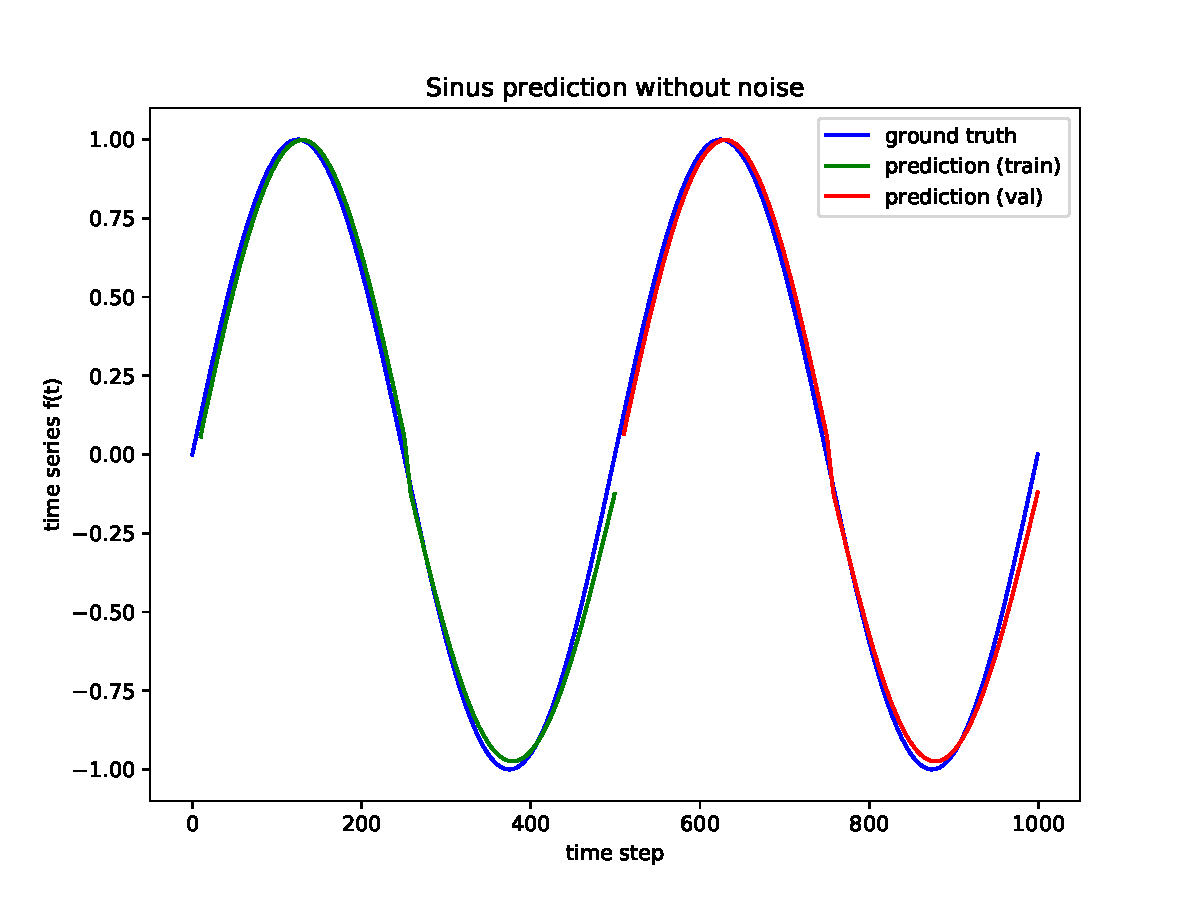
\includegraphics[width=\linewidth]{figures/plot_twolayer_noiseless.pdf}
  \end{subfigure} 
  \hspace{-5mm}
  \begin{subfigure}{.35\textwidth}
    \centering
    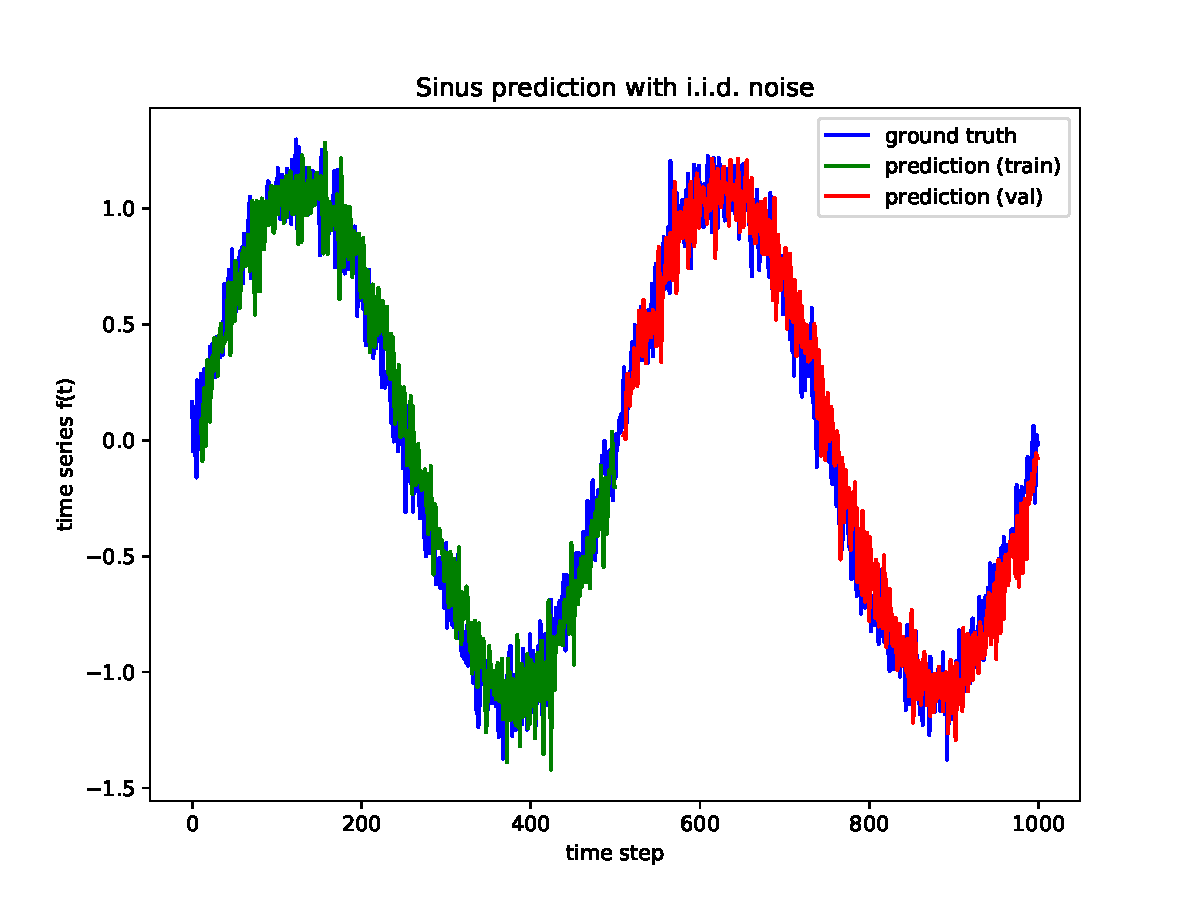
\includegraphics[width=\linewidth]{figures/plot_twolayer_iidnoise.pdf}
  \end{subfigure} 
  \hspace{-5mm}
  \begin{subfigure}{.35\textwidth}
    \centering
    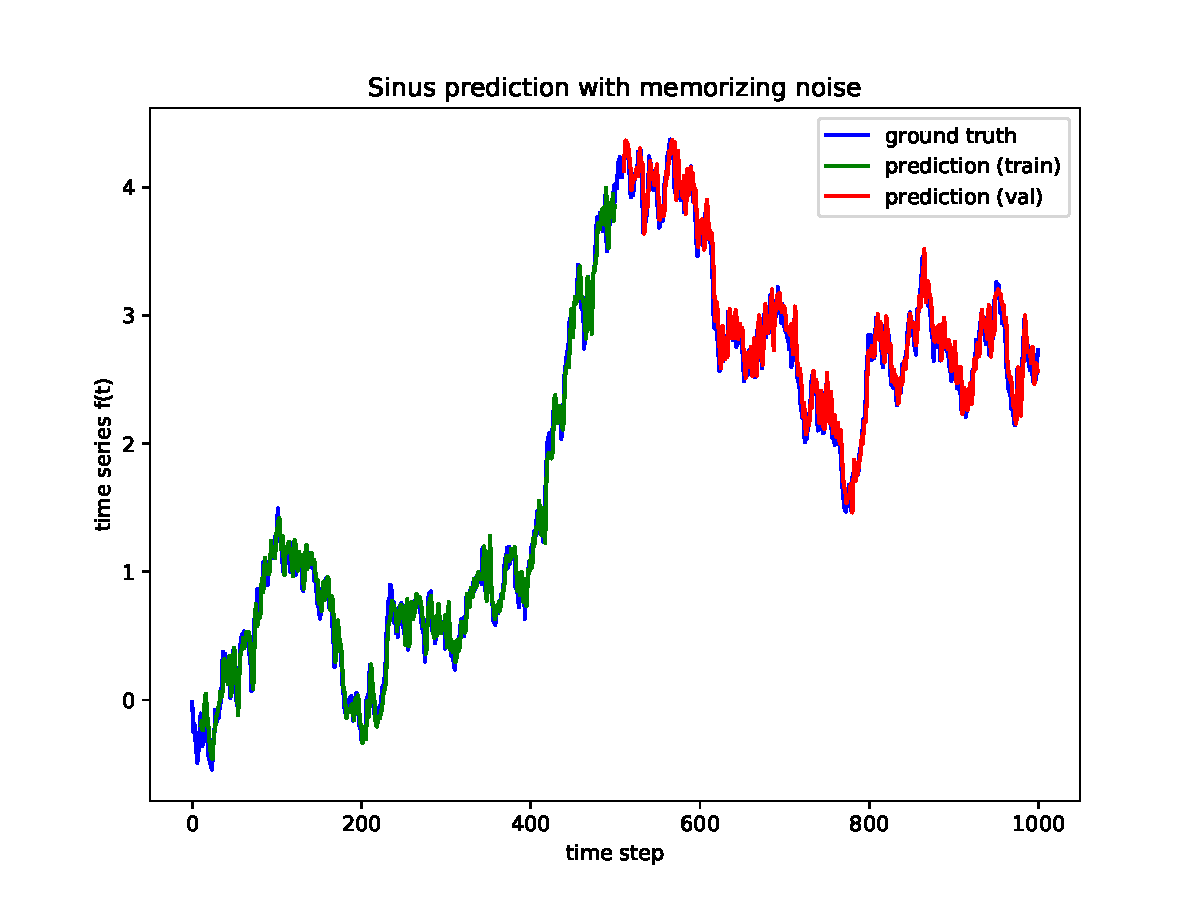
\includegraphics[width=\linewidth]{figures/plot_twolayer_memnoise.pdf}
  \end{subfigure}
  \caption{Impact of different kinds of noise on the time series prediction
  using a feedforward neural network with one hidden layer. Number of hidden
  units stays 10 in all simulations. Gaussian distributed noise with $\sigma = 
  0.1$.}
  \label{fig:noise_impact} 
\end{figure}

\begin{figure}
  \center
  \begin{subfigure}{.35\textwidth}
    \centering
    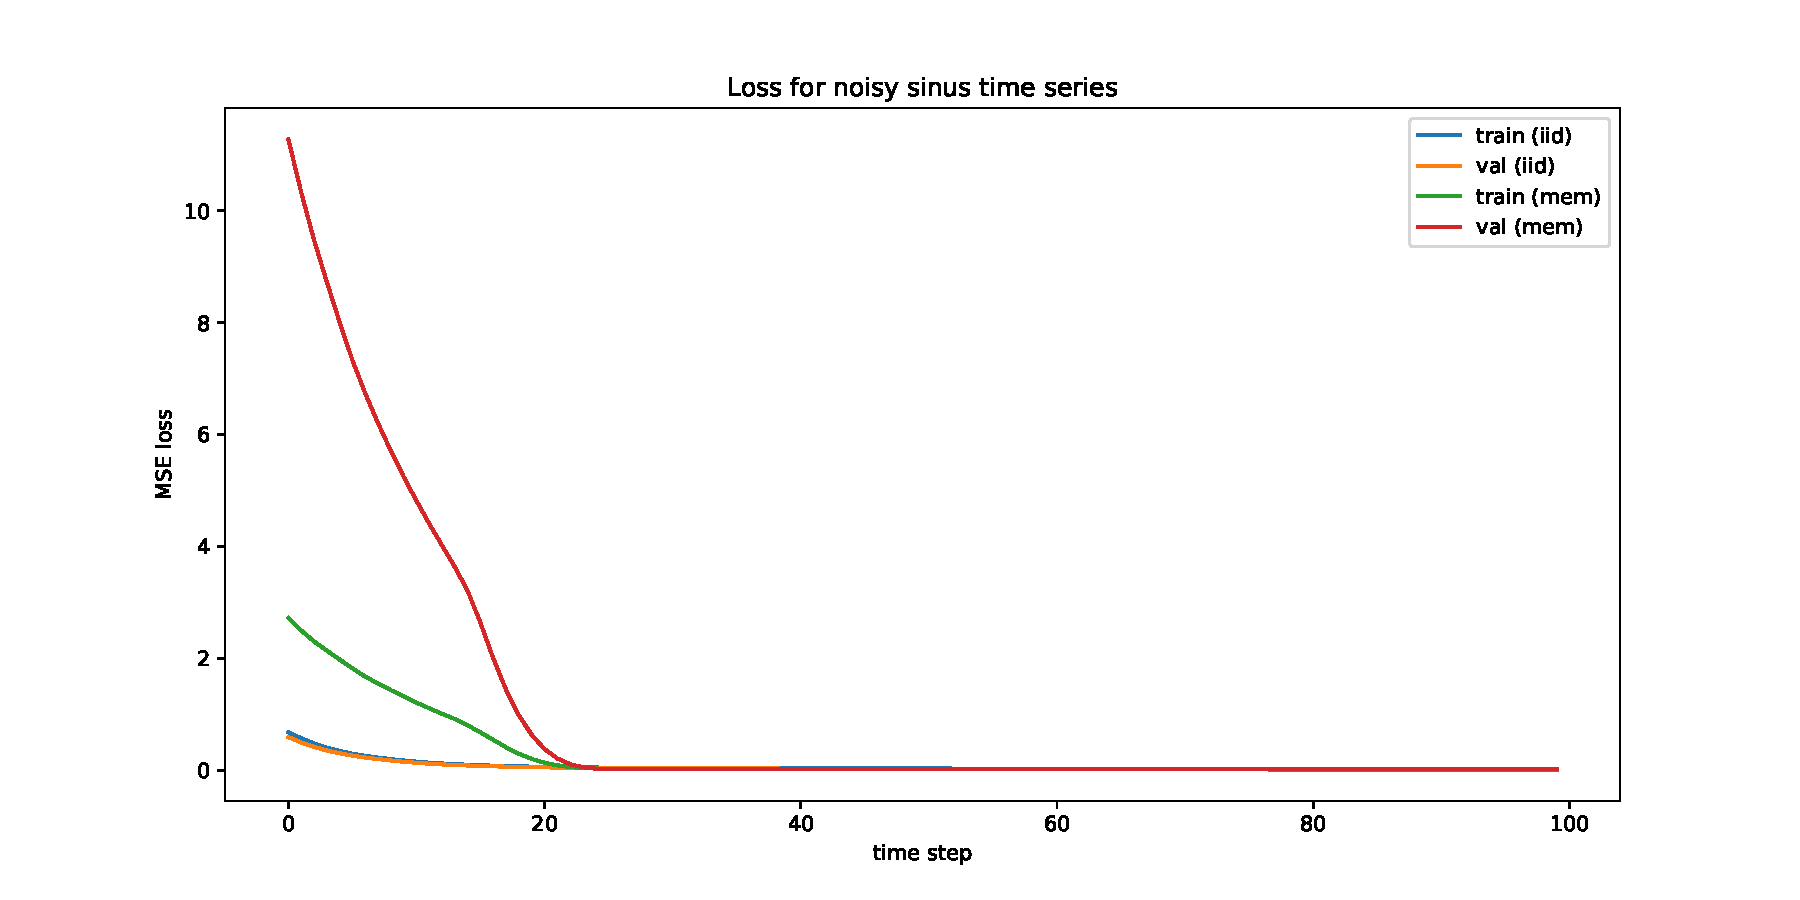
\includegraphics[width=\linewidth]{figures/plot_twolayer_losscompare.pdf}
  \end{subfigure} 
  \hspace{-6mm}
  \begin{subfigure}{.35\textwidth}
    \centering
    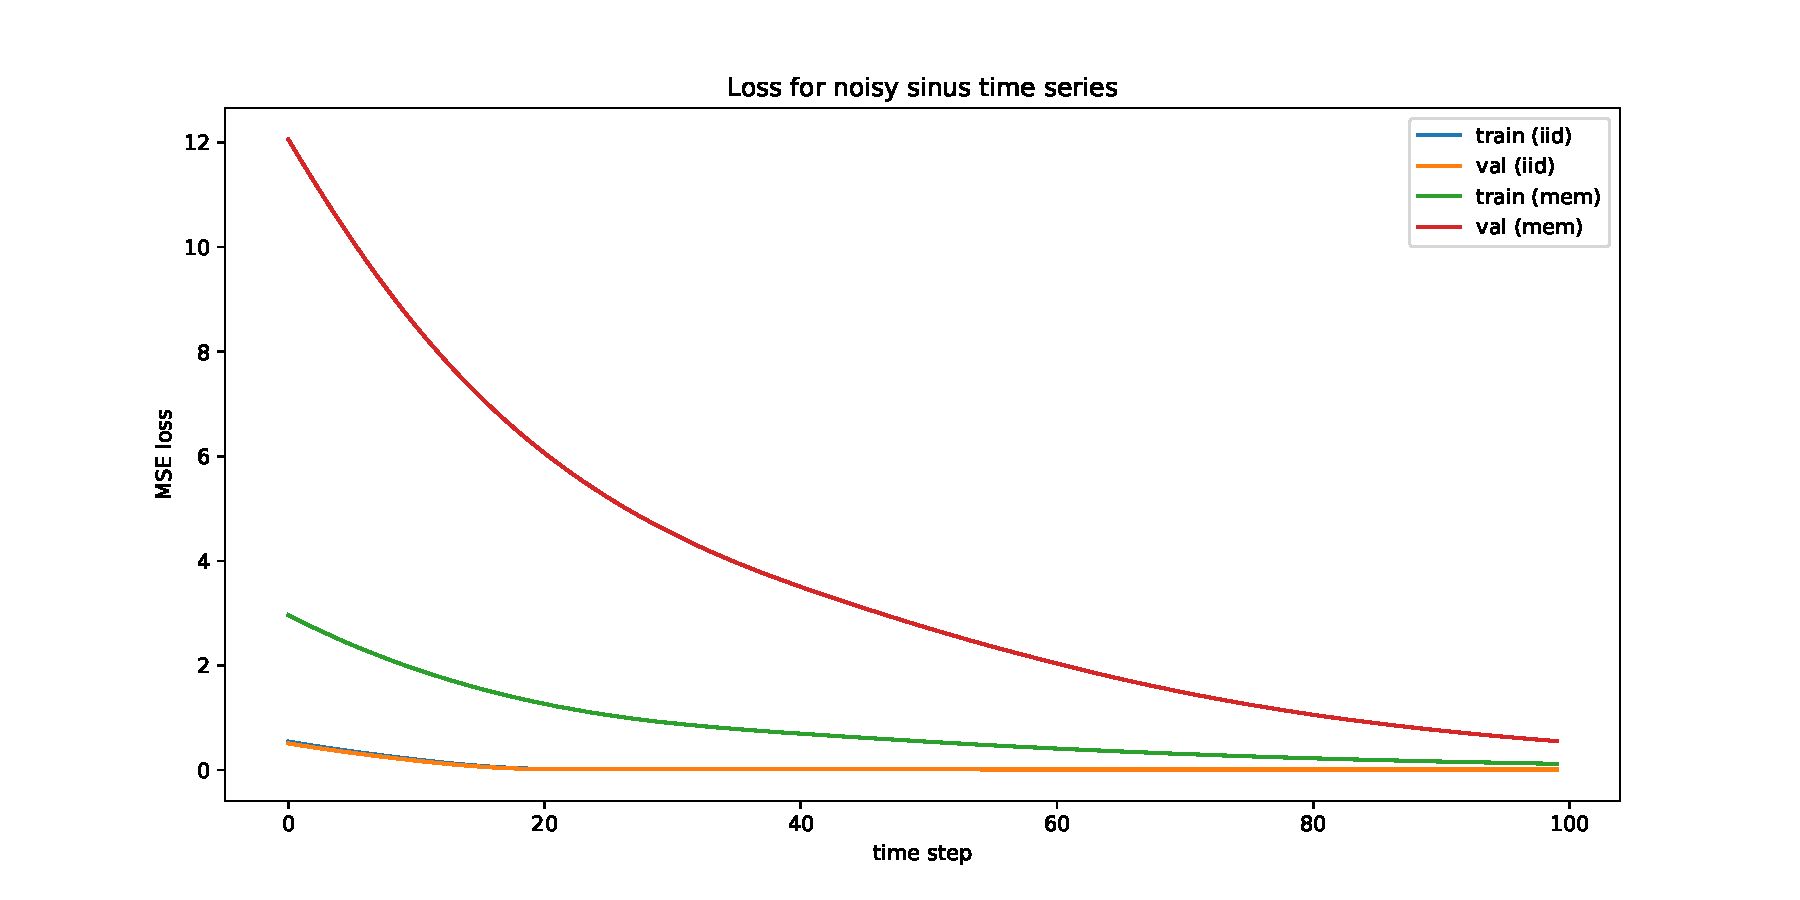
\includegraphics[width=\linewidth]{figures/plot_lstm_losscompare.pdf}
  \end{subfigure} 
  \hspace{-6mm}
  \begin{subfigure}{.35\textwidth}
    \centering
    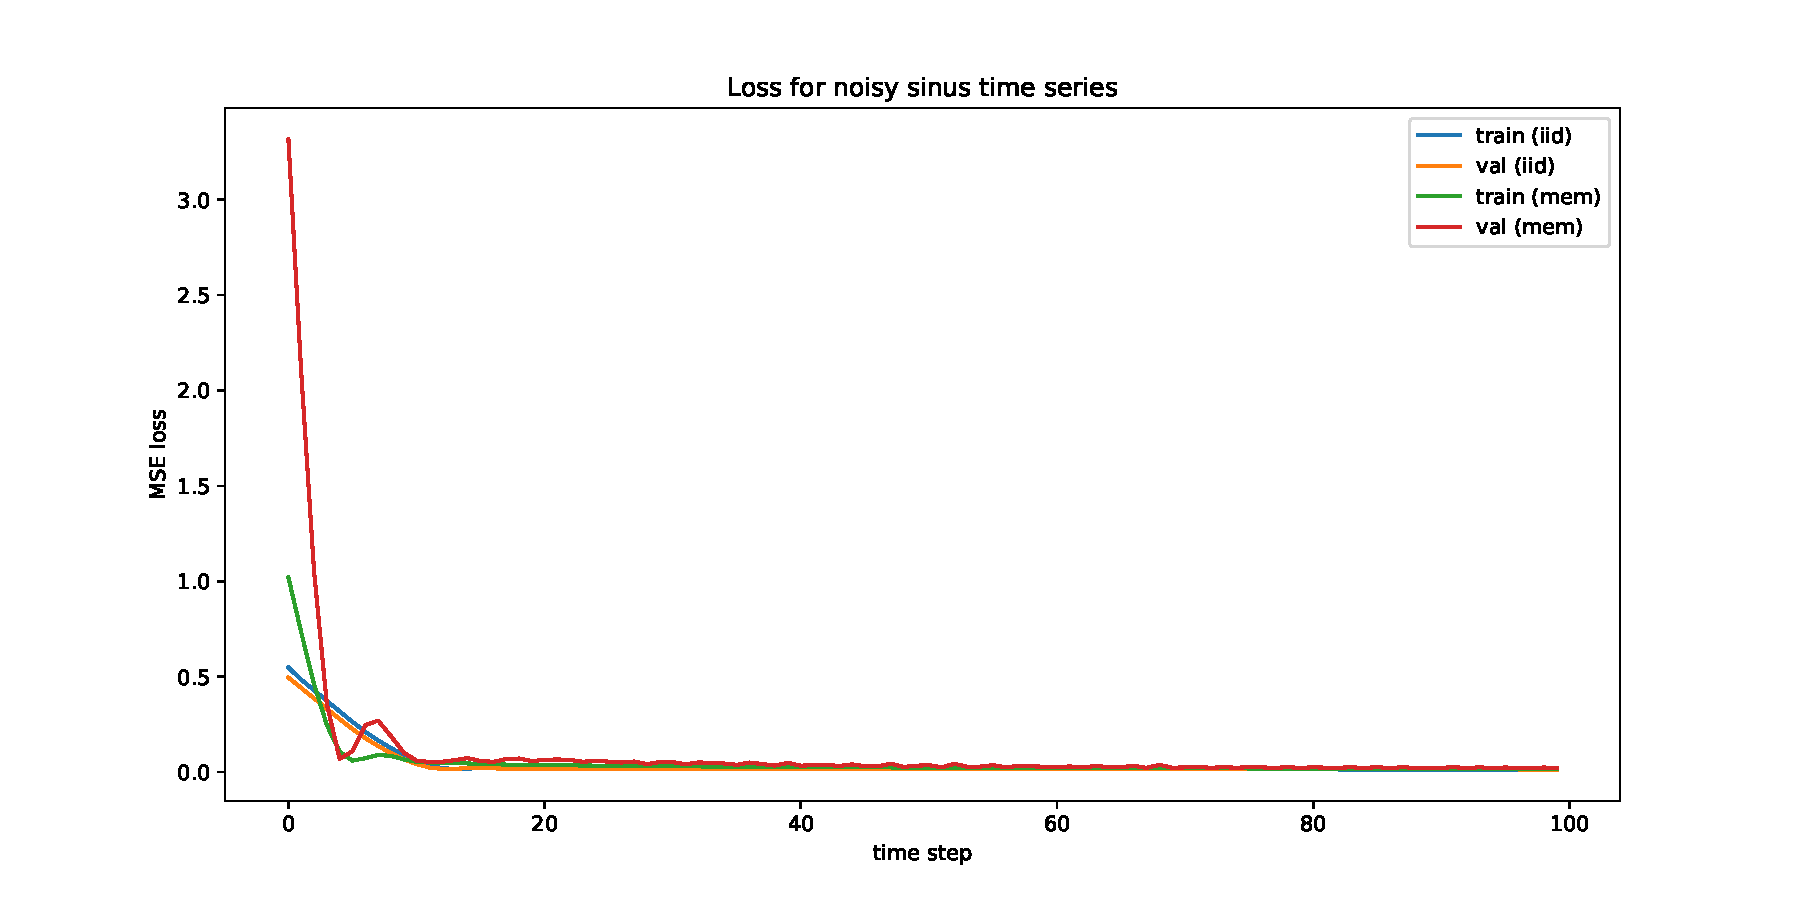
\includegraphics[width=\linewidth]{figures/plot_cnn_losscompare.pdf}
  \end{subfigure}
  \caption{MSE loss over the number of trained epochs on training and on 
  validation dataset. On the left, the classical feedforward network was used.
  The middle plot shows the performance of the LSTM and the right one plots the
  loss values of the convolutional network.}
  \label{fig:noise_loss_impact}
\end{figure}

% todo: advanced feature preparation
\subsection{Mackey Glass time series forecasting}

In order to model diseases related to dynamic respiratory and hematopoietic
diseases, Mackey \textit{et al.} proposed the mackey-glass equations, a kind of
first-order nonlinear differential delay equations to model 
the number of white blood cells over time \cite{mackey1977}. If the
delayed time ($x_{\tau} = x(t - \tau)$) exceeds the delay $\tau > 16.8$, then
equation \ref{equ:mackey} behaves chaotic \cite{farmer1982}.

\begin{equation}
  \frac{dx}{dt} = \beta \cdot \frac{x_{\tau}}{1 + x_{\tau}^n}
  \label{equ:mackey}
\end{equation}

The first approach to predict the short-time behavior of chaotic time series
was done by Farmer \textit{et al.} who proposed a \texttt{local approximation}
technique \cite{farmer1987}. After improval of predictions using support vector
machines by Müller \textit{et al.} \cite{muller1997}, the focus in research
shifted towards artifical neural networks which enable even better predictions.
Two of the latest developments are the usage of Wavelet Networks
\cite{alexandridis2013} and particle swarm optimization \cite{caraballo2016}.

The solution to the Mackey Glass equation is discretized using the Euler method,
as given in Equation~\ref{equ:mackey_euler}. using this discretisation we can
see the chaotic nature of the solution by comparing the time series evolution 
in
Figure~\ref{fig:mackey_chaos}. It can be seen clearly that the chaotic behavior
of the system gets stronger when the time delay is increased.

\begin{equation}
  x(t+1) = x(t) + \frac{\beta x(t - \tau)}{1 + x^{n}(t - \tau)} - \gamma x(t)
  \label{equ:mackey_euler}
\end{equation}

\begin{figure}
  \centering
  \begin{subfigure}{.5\textwidth}
    \centering
    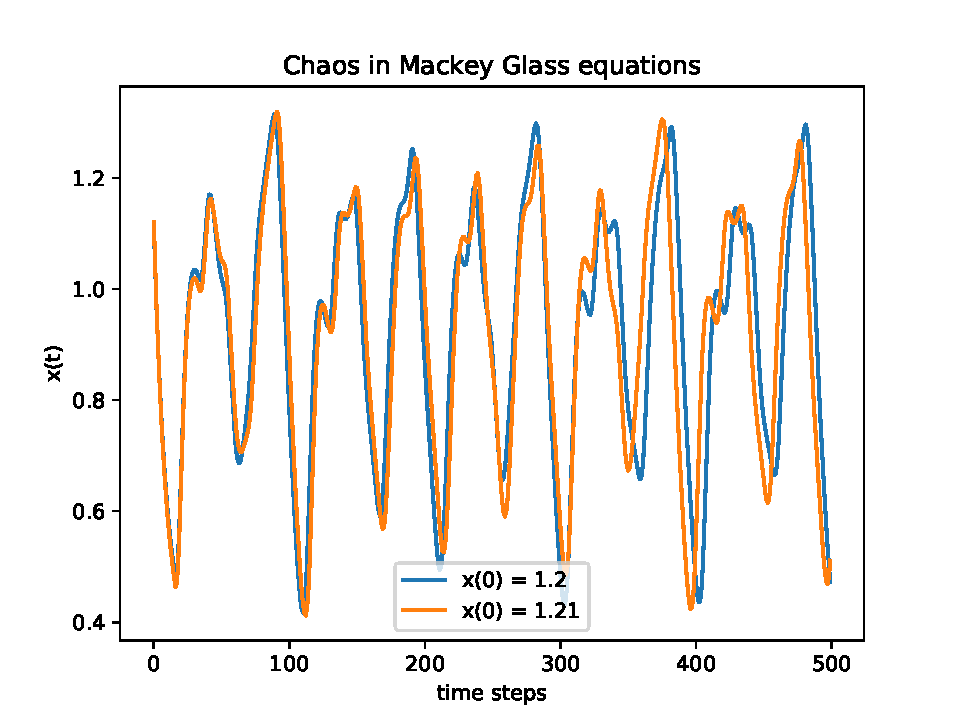
\includegraphics[width=\linewidth]{figures/mg_chaos_17.pdf}
  \end{subfigure} 
  \hspace{-6mm}
  \begin{subfigure}{.5\textwidth}
    \centering
    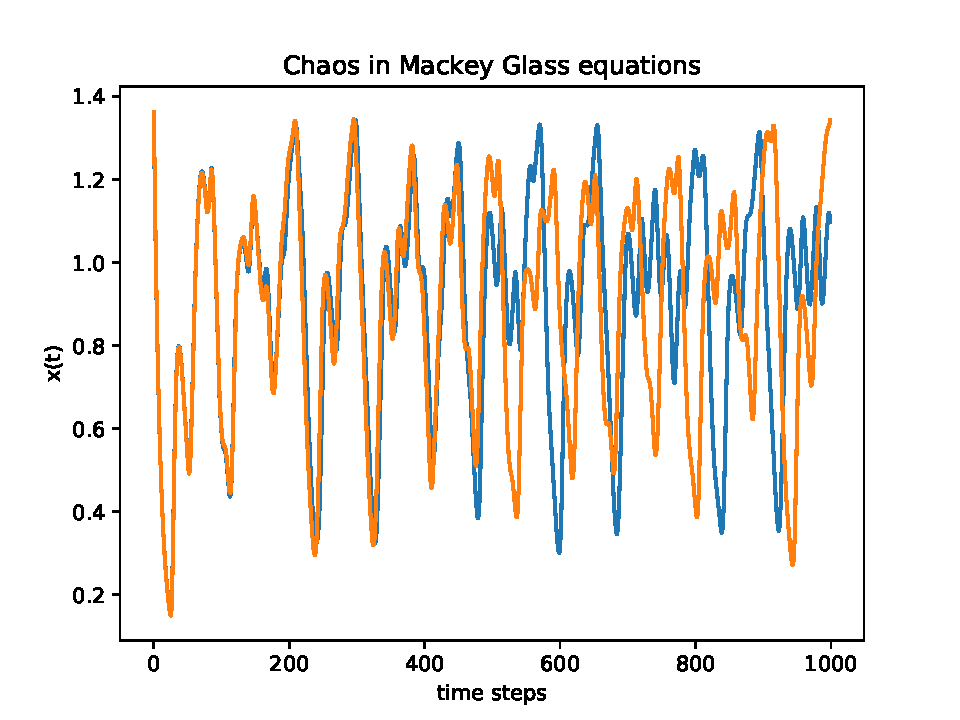
\includegraphics[width=\linewidth]{figures/mg_chaos_25.pdf}
  \end{subfigure}
  \caption{Influence of time delay parameter $\tau$ on the chaotic behavior of
    the Mackey Glass equation. The left side of the figure uses $\tau = 17$,
    the right side $\tau = 25$.}
  \label{fig:mackey_chaos}
\end{figure}

In accordance with the approach used by Caraballo \textit{et al.}
\cite{caraballo2016}, we predict $x(t+6)$ based on the information of the time 
series points in $x(t)$, $x(t-6)$, $x(t-12)$, and $x(t-18)$. We investigate how
an increase in chaotic behavior impacts the prediction capability of the
different neural network architectures. The results for the feedforward neural
network are depicted in Figure~\ref{fig:mackey_cnn}. For this plot, a 2-layer 
CNN architecture was used, incoroporating "same" padding and a kernel size of 3.
The first 3000 time points of the time series are used for training, the 1000 
following points for validation.

It can be seen that for non-chaotic solutions of the macke-glass time series the
model is able to predict precisely, and that for values of $\tau > 20$ the 
chaotic behavior is strong enough to impact the prediction. We explain the low
error for $\tau = 21$ in the ability of the network to compensate for the amount
of chaos up to this point.
 
\begin{figure}
  \centering
  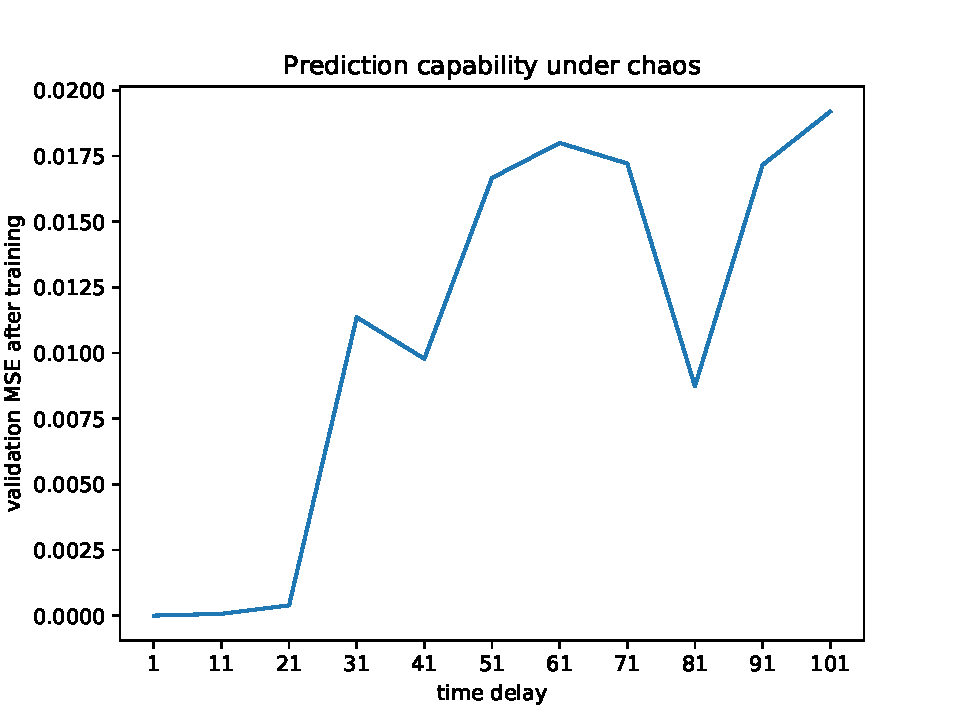
\includegraphics[width=0.6\textwidth]{figures/mackey_glass_cnn.pdf}
  \label{fig:mackey_cnn}
  \caption{Validation error of the convolutional neural network for different 
  time delay values $\tau$ of the Mackey Glass equation. The error increases 
  strongly for values of $\tau > 20$, indicating a strong chaotic behavior 
  from this point.}
\end{figure}

\subsection{Biological oscillator time series forecasting}

The next section deals with time series forecasting of biological oscillators, 
as described by Novak \textit{et al} \cite{novak2008}. For different aspects of
cell physiology, e.g. the DNA synthesis, this kind of oscillators can be 
observed. Novak \textit{et al} show that oscillations in simple ODEs can be 
produced by incorporating an explicit time delay \cite{novak2008}, similar to 
the Mackey Glass equations \cite{mackey1977}.

Recently, Strömstedt \textit{et al} analyzed the capability of neural network
architectures to model stochastic time series \cite{stroemstedt2018} at the 
example of time series produced according to the characteristics of Novak 
\textit{et al} \cite{novak2008}. In this section, we reproduce their results for
the LSTM architecture and show how to improve their results.

\section{Conclusion}

\bibliographystyle{alpha}
\bibliography{report}
\end{document}